\chapter{Dense-by-Sparse Algorithms}
\label{chapter:algs}

Why do we focus on this? 

Show the flowchart of different options

\begin{figure}[H]
  \centering
  

\usetikzlibrary{shapes,arrows}
\usetikzlibrary{decorations.pathreplacing}


% Define block styles
\tikzstyle{decision} = [diamond, draw, fill=blue!20, 
    text width=4.5em, text badly centered, node distance=3cm, inner sep=0pt]

\tikzstyle{block} = [rectangle, draw, fill=gray!20, 
    text width=7em, text centered, minimum height=3em]

\tikzstyle{line} = [draw, -latex']

\tikzstyle{cloud} = [draw, ellipse,fill=red!20, node distance=3cm,
    minimum height=2em]

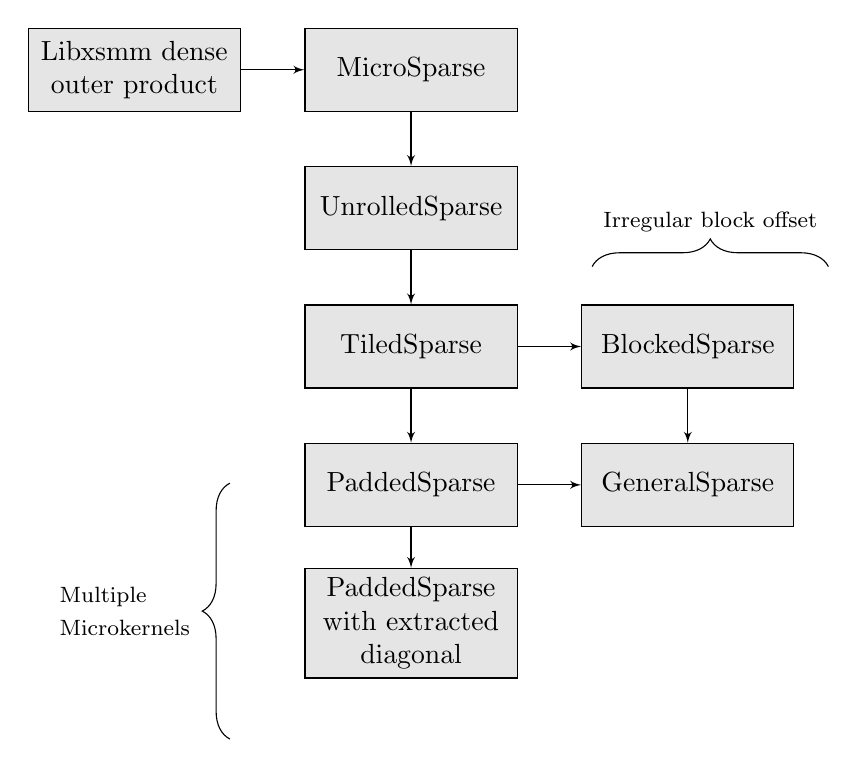
\begin{tikzpicture}[node distance = 5em, auto]
    % Place nodes

    \node [block] (microkernel) {MicroSparse};
    \node [block, left of=microkernel, node distance=10em] (libxsmm) {Libxsmm dense outer product};
    \node [block, below of=microkernel] (macrokernel) {UnrolledSparse};
    \node [block, below of=macrokernel] (tiledsparse) {TiledSparse};
    \node [block, right of=tiledsparse, node distance=10em] (blocksparse) {BlockedSparse};
    \node [block, below of=tiledsparse] (paddedsparse) {PaddedSparse};
    \node [block, below of=blocksparse] (generalsparse) {GeneralSparse};
    \node [block, below of=paddedsparse] (paddeddiagsparse) {PaddedSparse with extracted diagonal};

    %\node [block, left of=evaluate, node distance=3cm] (update) {update model};
    %\node [decision, below of=evaluate] (decide) {is best candidate better?};
    %\node [block, below of=decide, node distance=3cm] (stop) {stop};

    % Draw edges
    \path [line] (libxsmm) -- (microkernel);
    \path [line] (microkernel) -- (macrokernel);
    \path [line] (macrokernel) -- (tiledsparse);
    \path [line] (tiledsparse) -- (blocksparse);
    \path [line] (tiledsparse) -- (paddedsparse);
    \path [line] (paddedsparse) -- (generalsparse);
    \path [line] (blocksparse) -- (generalsparse);
    \path [line] (paddedsparse) -- (paddeddiagsparse);

    \draw [decorate,decoration={brace,amplitude=10pt},xshift=0pt,yshift=0pt]
(2.3,-2.5) -- (5.3,-2.5)node [black,midway,yshift=9pt] {\footnotesize Irregular block offset};

    \draw [decorate,decoration={brace,amplitude=10pt},xshift=0pt,yshift=0pt]
(-2.3,-8.5) -- (-2.3,-5.25) node [black,midway,xshift=-8pt,text width=5em] {\footnotesize Multiple\\ Microkernels};
    %\path [line] (evaluate) -- (decide);
    %\path [line] (decide) -| node [near start] {yes} (update);
    %\path [line] (update) |- (identify);
    %\path [line] (decide) -- node {no}(stop);
    %\path [line,dashed] (expert) -- (init);
    %\path [line,dashed] (system) -- (init);
    %\path [line,dashed] (system) |- (evaluate);
\end{tikzpicture}



  \label{fig:dxspfamilies}
  \caption{Relationships between different dense-by-sparse multiplication algorithms}
\end{figure}


\section{Sparse Microkernel}
Idea: Build off of the state of the art for small dense gemm
\begin{itemize}
    \item Assume A is dense, B is sparse
    \item Pack B into a virtual compressed-sparse-row or column format
    \item Remove all FMA and load instructions which are not needed
    \item Make this the basic building block for more complicated algorithms 
\end{itemize}

However, this has the following limitations:
\begin{itemize}
    \item Sparsity pattern must be known at compile time
    \item Pattern must fit within vector registers: $m \leq 8;  n \leq 30$
    \item (Dense $\times$ Sparse) $\neq$ (Sparse $\times$ Dense) due to vectorization
    \item Choice of row-major vs column-major format determines which of the two vectorizes nicely: $(AB)^T = B^T A^T$
\end{itemize}

\section{Unrolled dense-by-sparse multiplication}

Generate sparse microkernels for each (k,n) block of B, and unroll these into the instruction stream.
\begin{itemize}
      \item[$+$] Supports arbitrary matrix sizes
      \item[$+$] Dense-style register blocking for a dense $\times$ sparse algorithm.
      \item[$+$] Does not fill in any zeros -- no wasted flops

      \item[$-$] Generates an FMA instruction for each nonzero
      \item[$-$] These FMA instructions are 10B, too large to stream
      \item[$-$] Irregular location of blocks in memory prevents using tricks to reduce instruction size
      \item[$-$] Total number of nonzeros is limited by size of instruction cache.

\end{itemize}
\begin{figure}[ht]
      \begin{minted}[fontsize=\footnotesize]{text}
        {text}
        loop over m blocks:

           unroll loop over n blocks:

              load C block into registers

              unroll loop over k blocks:

                 load A block into registers
                 microkernel for current B block
                 move A right 1 block
                 move B down 1 block

              store C block from registers
              move A to far left
              move B to top + right 1 block
              move C right 1 block

           move A down 1 block
           move C down 1 block
      \end{minted}
\end{figure}


\section{Tiled dense-by-sparse multiplication}

        Assume there exists a sparse pattern which tiles perfectly over B.
        \begin{itemize}
        \item[$+$] We can reuse a single microkernel, reducing the number of instructions
        \item[$+$] We can visit blocks in a loop efficiently, using pointer tricks to reduce instruction size.
        \item[$-$] This regularity assumption is likely too strong.
        \item[$-$] In practice, the sparsity pattern would often become dense.
        \end{itemize}


      \[
      \left[
          \begin{array}{c c c | c c c }
          0 &   &   & 10 &   &   \\
          1 & 2 &   & 11& 12&   \\
            & 3 & 4 &   & 13& 14  \\
          \hline
          5 &   &   & 15  &   &   \\
          6 & 7 &   & 16  &17   &   \\
            & 8 & 9 &   & 18  &19   \\
          \end{array}
          \right]
      \]

\section{Block dense-by-sparse multiplication}

  Assume that B is decomposed into blocks which are either empty or `full'. `Full' blocks all have the same sparsity pattern. This is a sparse generalization of the block-sparse-column format.

  \begin{itemize}
  \item[$+$] We can reuse a single microkernel, reducing the number of instructions
  \item[$+$] The zero blocks reduce the number of filled-in nonzeros.
  \item[$-$] We can no longer visit blocks by using a loop with pointer arithmetic. \\Our options are:
    \begin{itemize}
    \item Look up the block location from a table in memory
    \item Unroll the block locations into the instruction stream and repeatedly jump to the microkernel.
    \end{itemize}
  \end{itemize}

      \[
      \left[
          \begin{array}{c c c | c c c }
          0 &   &   &    &    &    \\
          1 & 2 &   &    &    &    \\
            & 3 & 4 &    &    &    \\
          \hline
          5 &   &   & 10 &    &    \\
          6 & 7 &   & 11 & 12 &    \\
            & 8 & 9 &    & 13 & 14 \\
          \end{array}
          \right]
      \]
\section{General dense-by-sparse multiplication}
\section{Dense-by-sparse multiplication with an extracted diagonal}
